% Originally: content/week-02.tex, the second half of \section{Open and closed sets}
% (Corsin Week 2, Monday) --- promoted to a section of its own, since the chapter
% otherwise consisted of one section carrying the chapter's own title.
\section{Interior, closure and boundary}
\label{sec:interior_closure_boundary}

% Sonnet 5 (Medium)
\begin{definition}[Interior, closure, and boundary]
\label{def:interior_closure_boundary}
Let $(X,d)$ be a metric space and $A \subseteq X$. The \newterm{interior}
(\germanterm{Inneres}) of $A$ is
\[\operatorname{int}(A) := \{x \in A : \exists\, r>0 \text{ such that } B_r(x) \subseteq A\},\]
the largest open subset of $X$ contained in $A$. The \newterm{closure} (\germanterm{Abschluss}) of
$A$ is
\[\overline{A} := \{x \in X : B_r(x) \cap A \neq \emptyset \text{ for all } r > 0\},\]
the smallest closed subset of $X$ containing $A$. The \newterm{boundary} (\germanterm{Rand}) of
$A$ is $\partial A := \overline{A} \setminus \operatorname{int}(A)$.
\end{definition}

\begin{aiexample}[Interior, Closure, and Boundary of an Interval]
% Generator: Gemini 3.6 Flash (Medium)
Applying \cref{def:interior_closure_boundary} to $A := (0,1] \subset \mathbb{R}$ under the
standard Euclidean metric:
\begin{itemize}
  \item The \textbf{interior} is $\operatorname{int}(A) = (0,1)$, the largest open set contained in $A$.
  \item The \textbf{closure} is $\overline{A} = [0,1]$, the smallest closed set containing $A$.
  \item The \textbf{boundary} is $\partial A = \overline{A} \setminus \operatorname{int}(A) = \{0, 1\}$.
\end{itemize}
Note that $1 \in A$ while $0 \notin A$: the boundary is not required to lie inside the set, nor
outside it. That is the point of defining it as a difference of two other sets rather than as
\qt{the edge of $A$}.
\end{aiexample}

% Generator: Claude Opus 5 (High) --- FIG-W02-01: the three notions in one picture.
\begin{center}
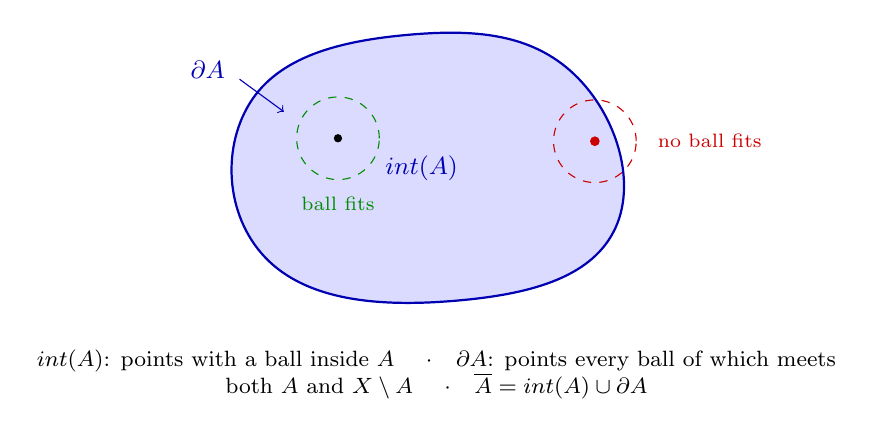
\begin{tikzpicture}[scale=1.25]
  % A blob A. int(A) is the shaded open part; the solid curve is dA; closure = both together.
  \draw[blue!70!black, thick, fill=blue!14, smooth cycle, tension=0.75]
    plot coordinates {(-1.7,-0.9) (-1.9,0.7) (-0.3,1.4) (1.4,1.0) (1.8,-0.6) (0.2,-1.3)};

  \node[blue!70!black, font=\small] at (-0.15,0.05) {$\operatorname{int}(A)$};

  % a point of the interior, with a ball that fits
  \fill (-1.0,0.35) circle (1.2pt);
  \draw[green!55!black, dashed] (-1.0,0.35) circle (0.42);
  \node[green!55!black, font=\scriptsize, below] at (-1.0,-0.15) {ball fits};

  % a boundary point: every ball meets A and its complement
  \fill[red!80!black] (1.61,0.32) circle (1.4pt);
  \draw[red!80!black, dashed] (1.61,0.32) circle (0.42);
  \node[red!80!black, font=\scriptsize, anchor=west] at (2.15,0.32) {no ball fits};

  \node[blue!70!black, font=\small, anchor=east] at (-2.05,1.05) {$\partial A$};
  \draw[blue!70!black, ->] (-2.0,0.95) -- (-1.55,0.62);

  \node[font=\footnotesize, align=center] at (0,-2.05)
    {$\operatorname{int}(A)$: points with a ball inside $A$ \quad$\cdot$\quad
     $\partial A$: points every ball of which meets\\
     both $A$ and $X\setminus A$ \quad$\cdot$\quad
     $\overline{A} = \operatorname{int}(A) \cup \partial A$};
\end{tikzpicture}
\end{center}

\begin{remark}[Interior and closure are dual]
\label{rem:interior_closure_dual}
The two constructions are not independent: taking complements swaps them,
\[X \setminus \operatorname{int}(A) = \overline{X\setminus A},
  \qquad\qquad
  X \setminus \overline{A} = \operatorname{int}(X\setminus A).\]
Both read off \cref{def:interior_closure_boundary} directly, since $x$ fails to have a ball inside
$A$ exactly when every ball around $x$ meets $X\setminus A$. In particular $\partial A =
\partial(X\setminus A)$: a set and its complement share their boundary, which is why the
boundary of the open disk and of its closed complement are the same circle.
\end{remark}

% Source: Corsin Nick/Class Notes/Week 2.pdf, p. 7
\begin{exercise}[$X$ and $\emptyset$ are clopen]
\label{ex:X_empty_clopen}
Let $(X,d)$ be a metric space. Show that $X$ and $\emptyset$ are both open and closed.
\end{exercise}

% Kept inline: solved directly in Corsin Nick/Class Notes/Week 2.pdf, p. 7.
\begin{exercisesolution}[Proof of \cref{ex:X_empty_clopen}]
$X$ is open, since $B_r(x) \subseteq X$ for all $r > 0$ and $x \in X$
(\cref{def:open_ball}). The empty set contains no
points and is therefore vacuously open. Since $X$ and $\emptyset$ are each other's complement in
$X$, they are also closed.
\end{exercisesolution}

% Supplement: Sascha Brack/Class Notes/Week_02_Notes_Friday_Updated.pdf, p. 2
\begin{example}[Interior, closure, and boundary in $\mathbb{R}$ and $\mathbb{R}^2$]
\label{ex:interior_closure_boundary_more}
Applying \cref{def:interior_closure_boundary} to various sets:
\begin{enumerate}[label=\textbf{(\alph*)}]
  \item Let $\Omega := \mathbb{Z} \subset \mathbb{R}$. Then $\operatorname{int}(\Omega) = \emptyset$ (no interval fits inside $\mathbb{Z}$), $\overline{\Omega} = \mathbb{Z}$ (it is already closed), and $\partial\Omega = \mathbb{Z} \setminus \emptyset = \mathbb{Z}$.
  \item Let $\Omega := B_1(0) \subset \mathbb{R}^2$. Then $\operatorname{int}(\Omega) = B_1(0)$ (it is already open), the closure is the closed disk $\overline{\Omega} = \{x \in \mathbb{R}^2 \mid d(x,0) \leq 1\}$, and the boundary is the unit circle $\partial\Omega = \{x \in \mathbb{R}^2 \mid d(x,0) = 1\}$.
  \item Let $\Omega := \mathbb{Q} \subset \mathbb{R}$. Then $\operatorname{int}(\Omega) = \emptyset$ (every open interval contains irrationals), $\overline{\Omega} = \mathbb{R}$ (every open interval contains rationals, so every real number is a closure point), and $\partial\Omega = \mathbb{R} \setminus \emptyset = \mathbb{R}$.
\end{enumerate}
\end{example}

% Supplement: Analysis_II_Script_v1.pdf, p. 15
\begin{exercise}[Closure and boundary of a ball in $\mathbb{R}^n$]
\label{ex:closure_boundary_of_ball}
For balls $B_r(x)$ in $\mathbb{R}^n$ with the Euclidean metric, prove that
\[\overline{B_r(x)} = \{y \in \mathbb{R}^n : d(x,y) \leq r\}\]
and deduce $\partial B_r(x) = \{y \in \mathbb{R}^n : d(x,y) = r\}$.
\end{exercise}

\begin{remark}
Item \textbf{(b)} of \cref{ex:interior_closure_boundary_more} above is exactly the case $r=1$,
$x=0$, $n=2$ of this exercise, worked here for general $x$, $r$ and $n$.
\end{remark}

% Quelle: Jérôme Paschoud/Notizen/Woche 2.1 Metrische Räume.pdf, p. 6
\begin{exercise}[Interior, closure, and boundary of a mixed set]
\label{ex:interior_closure_boundary_mixed}
Let $E := (\{0\} \times \mathbb{R}) \cup (0,1)^2 \subset \mathbb{R}^2$. Find the interior $\operatorname{int}(E)$, the closure $\overline{E}$, and the boundary $\partial E$ with respect to the standard metric on $\mathbb{R}^2$.
\end{exercise}

% Generator: Gemini 3.6 Pro
\begin{exercisesolution}[Proof of \cref{ex:interior_closure_boundary_mixed}]
\begin{itemize}
  \item \textbf{Interior:} $\operatorname{int}(E) = (0,1)^2$. The line $\{0\} \times \mathbb{R}$ contains no 2D open balls, so it contributes nothing to the interior. The open square $(0,1)^2$ is already open in $\mathbb{R}^2$.
  \item \textbf{Closure:} $\overline{E} = (\{0\} \times \mathbb{R}) \cup [0,1]^2$. The line $\{0\} \times \mathbb{R}$ is closed. The closure of the open square is the closed square $[0,1]^2$. The closure of a finite union is the union of the closures.
  \item \textbf{Boundary:} $\partial E = \overline{E} \setminus \operatorname{int}(E) = (\{0\} \times \mathbb{R}) \cup \big([0,1]^2 \setminus (0,1)^2\big)$. The second term is the perimeter of the square.
\end{itemize}
\end{exercisesolution}
